\section{Münsterrätsel}
Im Folgenden seht ihr fünf Verkehrsschilder aus Münster.
Wer von euch es zuerst schafft, bis zum 31.~Oktober vier von fünf Schildern an ihrem Platz zu fotografieren, bekommt einen Preis.
Dieser kann im Fachschaftsraum abgeholt werden.

\begin{center}
	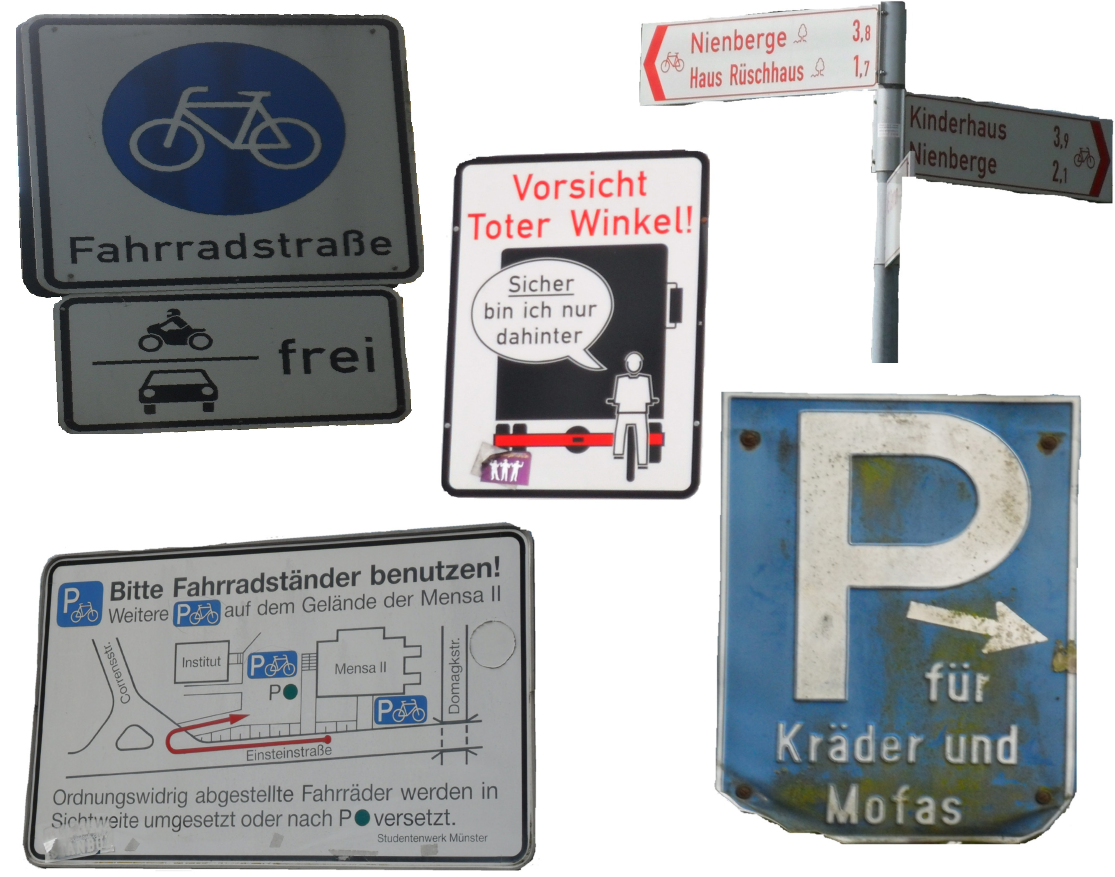
\includegraphics[width=\textwidth, height=0.55\textheight]{res/muensterraetsel_schilder.pdf}
\end{center}

\section*{Fortsetzung Münsterrätsel}
In diesem Rätsel findet ihr waagerecht, senkrecht und diagonal (l.\ o.\ nach r.\ u.) die wichtigsten Kneipen und Discos in Münster, die ihr kennen solltet.
Viel Spaß beim Suchen! (Tipp: Insgesamt haben wir 36~Namen versteckt.)
\begin{center}
	\footnotesize
	% Horizontales Padding in der Tabelle einstellen
	\setlength{\tabcolsep}{0.3em}
	\begin{tabular}{| *{29}{>{\centering\arraybackslash}m{1.1em} |}}
		\hline
		B & C & F & R & H & Ü & T & G & J & E & R & W & H & T & P & M & H & E
			& I & B & W & A & T & U & S & I & B & A & R
		\\ \hline
		C & U & D & F & E & G & D & O & E & D & E & A & D & E & Z & K & P & R
			& G & L & G & C & I & N & E & P & S & A & F
		\\ \hline
		A & B & H & E & A & S & E & R & D & F & R & L & E & R & Ä & Ä & S & I
			& H & O & T & J & A & Z & Z & C & L & U & B
		\\ \hline
		N & A & B & W & V & Z & A & I & R & D & U & N & G & U & R & A & K & D
			& E & D & H & E & E & J & K & D & A & H & V
		\\ \hline
		E & C & D & E & E & F & W & L & I & G & C & L & U & B & P & A & L & M
			& A & W & R & R & M & G & O & M & H & E & U
		\\ \hline
		F & L & B & A & N & M & X & L & T & B & E & A & E & W & N & E & L & E
			& W & V & T & V & S & D & M & V & X & U & N
		\\ \hline
		F & U & T & F & W & T & N & A & U & R & J & E & V & I & U & Z & A & U
			& W & U & I & N & I & A & W & S & E & G & G
		\\ \hline
		J & B & U & K & E & A & P & B & N & B & U & D & D & E & N & T & U & R
			& M & R & S & D & E & S & T & I & L & L & E
		\\ \hline
		C & G & M & U & U & R & M & A & M & U & C & I & E & M & T & T & W & E
			& U & E & A & H & W & N & Y & H & Z & E & S
		\\ \hline
		T & N & R & D & S & I & A & R & E & L & N & H & H & M & N & E & L & H
			& Ö & M & L & E & Z & A & S & G & I & I & E
		\\ \hline
		X & L & L & K & B & A & R & C & E & L & O & N & A & Z & Ö & I & H & U
			& M & W & E & B & T & L & C & B & E & S & R
		\\ \hline
		M & X & I & S & L & E & I & E & I & E & B & D & I & G & H & E & I & L
			& E & W & E & L & T & P & H & H & G & Z & T
		\\ \hline
		Z & F & T & G & A & S & O & L & I & N & M & R & F & B & J & F & F & T
			& I & I & I & J & R & O & W & S & E & W & U
		\\ \hline
		H & H & U & I & G & B & E & U & R & K & R & E & I & E & A & N & K & P
			& A & O & U & F & S & U & A & N & W & E & B
		\\ \hline
		D & J & F & E & E & A & J & D & E & O & N & D & S & I & F & U & L & I
			& Z & Ö & J & U & M & Y & R & D & M & I & P
		\\ \hline
		S & R & E & D & H & S & Z & L & Z & P & I & Q & C & K & J & N & E & O
			& Q & D & T & R & D & M & Z & I & B & U & L
		\\ \hline
		N & T & D & G & A & Z & Ü & E & P & P & E & E & H & F & E & I & U & N
			& F & E & O & E & E & Z & E & S & A & N & A
		\\ \hline
		P & I & N & K & U & S & M & Ü & L & L & E & R & B & E & N & C & H & I
			& L & A & D & A & N & S & S & R & R & D & N
		\\ \hline
		U & N & W & K & S & A & F & U & W & L & R & F & A & U & E & Q & E & M
			& S & P & O & O & K & Y & S & I & Z & Z & B
		\\ \hline
		Z & I & E & W & K & U & A & E & U & I & E & J & R & E & I & M & S & D
			& M & Z & P & U & M & S & C & N & I & W & A
		\\ \hline
		E & V & T & U & S & E & U & I & M & E & I & U & A & S & K & U & L & K
			& F & A & F & A & E & A & H & K & L & A & E
		\\ \hline
		E & D & D & Y & S & B & A & R & A & M & H & A & F & E & N & E & L & E
			& U & N & J & G & E & R & A & T & L & N & T
		\\ \hline
		P & Z & D & V & I & M & E & A & N & Z & E & T & Y & M & D & R & E & T
			& S & W & E & S & Z & R & F & U & U & Z & I
		\\ \hline
		D & A & S & B & L & A & U & E & H & A & U & S & N & V & M & O & T & Z
			& I & O & R & Z & U & R & X & W & S & I & O
		\\ \hline
		T & C & O & C & O & N & U & T & B & E & A & C & H & I & O & T & A & E
			& O & J & H & R & M & A & T & O & N & G & P
		\\ \hline
		U & T & K & O & M & P & A & H & U & H & T & Z & E & H & C & E & I & T
			& N & T & R & I & P & T & Y & C & H & O & N
		\\ \hline
		B & B & J & C & L & U & B & F & A & V & E & L & A & W & A & L & W & D
			& Q & D & T & M & S & R & D & G & E & O & G
		\\ \hline
		S & C & F & S & A & T & D & D & E & A & R & W & M & A & M & O & E & F
			& D & T & D & A & S & C & E & A & V & N & S
		\\ \hline
		S & A & L & S & O & M & A & N & I & A & E & W & P & C & B & L & A & B
			& E & M & I & E & Z & R & I & O & R & E & N
		\\ \hline
		T & V & F & G & H & R & S & E & Z & S & Ü & E & Z & C & O & A & S & P
			& U & T & N & I & K & H & A & L & L & E & Y
		\\ \hline
	\end{tabular}
	
	\includegraphics[width=\textwidth, height=0.25\textheight]{private/res/comics/darts.pdf}
	\rotatebox{90}{
		\tiny
		\hrefurl{http://www.dartsport-rostock.de/dartsport_rostock_lustiges.html}{www.dartsport-rostock.de/dartsport\_rostock\_lustiges.html}
	}
\end{center}

\vspace{-3ex}
\fibelsig{Simon}

\clearpage

\subsection{Überlebenstraining für Physiker in Münster}
\begin{multicols}{2}
\textbf{Die Antworten auf die folgenden Fragen könnten für euch im Verlaufe eures Studiums absolut lebensnotwendig werden\dots\ oder auch nicht!}

\newlist{fibelanswer}{enumerate}{1}
\setlist[fibelanswer]{
	label=\alph*),
	parsep=0.6ex,
	before=\normalfont,
	after=\vspace{0.8ex}
}
\begin{enumerate}[before=\itshape\RaggedRight]
	\item Wie wird Münsters erste akademische Bieranstalt genannt?
	\begin{fibelanswer}
		\item Destille
		\item Cavete
		\item Das Blaue Haus
		\item Pinkus Müller
	\end{fibelanswer}
	\label{itm:rätsel_bieranstalt}
	\item Welche chemische Verbindung sorgt dafür, dass man am Aasee-Ufer ohne Atemschutzmaske joggen/grillen kann?
	\begin{fibelanswer}
		\item \ch{Fe(II)Cl}
		\item \ch{Fe(III)Cl}
		\item \ch{C_2H_5OH}
		\item \ch{H_1N_1}
	\end{fibelanswer}
	\label{itm:rätsel_ethanol}
	\item Welche Wochentage gehen auf Namen germanischer Götter zurück?
	\begin{fibelanswer}
		\item Dienstag, Donnerstag, Freitag
		\item Dienstag, Mittwoch, Donnerstag
		\item Donnerstag, Freitag, Samstag
		\item Alle
	\end{fibelanswer}
	\label{itm:rätsel_götter}
	\item "$\Xi$" -- Hä, Was ist denn das?
	\begin{fibelanswer}
		\item Xi
		\item Psi
		\item Chi
		\item Omikron
	\end{fibelanswer}
	\label{itm:rätsel_xi}
	\item Welcher Weg von der IG1 zur Ringmensa ist der schnellste?
	\begin{fibelanswer}
		\item Links um die Baustelle rum
		\item Rechts um die Baustelle rum
		\item Die Arbeiter anbetteln einen durch die Baustelle zu lassen
		\item Privathelikopter
	\end{fibelanswer}
	\label{itm:rätsel_mensa}
	\columnbreak
	\item Was entsteht auf der Baustelle neben der IG1?
	\begin{fibelanswer}
		\item IG0
		\item IG1
		\item IG2
		\item Badeparadies
	\end{fibelanswer}
	\label{itm:rätsel_baustelle}
	% XXX Jedes Jahr prüfen, ob der Preis noch stimmt!
	\item Warum sprudelt es an heißen Tagen im Aasee?
	\begin{fibelanswer}
		\item Belüftungsgeräte, die sauerstoffreiche und sauerstoffarme Wasserschichten für die Fische vermischen
		\item Um Besucher vom Baden abzuhalten
		\item Kunst aus dem Jahre 2017 im Rahmen der Skulptur Projekte
		\item Faulgase, die bei der Hitze aufsteigen
	\end{fibelanswer}
	\label{itm:rätsel_aasee}
	\item Welche Chemie-Formel kann sich kein Chemiker merken?
	\begin{fibelanswer}
		\item $n = \sfrac{m}{M}$
		\item $n M = m$
		\item $\sfrac{1}{n} = \sfrac{M}{m}$
		\item $\sfrac{n M}{m} = 1$
	\end{fibelanswer}
	\label{itm:rätsel_chemiker}
	\item Was kann man im Münsteraner Zoo füttern?
	\begin{fibelanswer}
		\item afrikanische Elefanten
		\item indische Elefanten
		\item asiatische Elefanten
		\item deutsche Elefanten
	\end{fibelanswer}
	\label{itm:rätsel_elefanten}
\end{enumerate}

\hfill(Lösung auf Seite \pageref{pg:rätsel_lösungen})

\begin{center}
	\includegraphics[width=.9\columnwidth, height=0.34\textheight]{private/res/nichtlustig/140729_hebel.jpg}
\end{center}
\end{multicols}
